\chapter{MANTA/SPIN} 
\label{sec:ships}
\lstset{style=6502Style}

When waiting to start the first level, the player's Manta ship spins elegantly in the
center of the screen. This simple animation uses an enormous number of sprites - 16 in
total. 
\begin{figure}[H]
    \centering
    \begin{adjustbox}{width=14cm,center}
      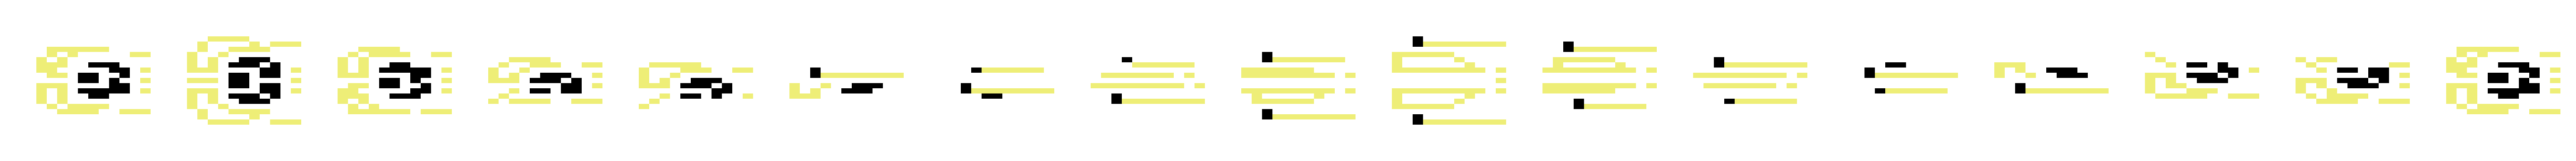
\includegraphics[width=15cm]{src/manta_spin/manta_spin.png}%
    \end{adjustbox}
\end{figure}
\vspace{-0.5cm}

The first phase of the spin -
\raisebox{-0.2\totalheight}{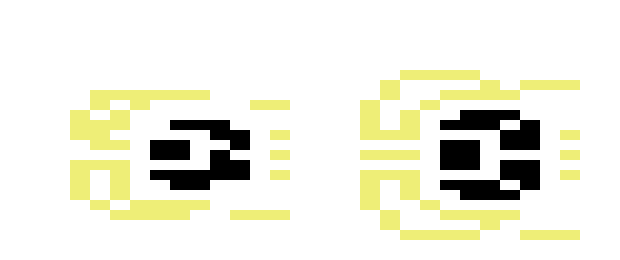
\includegraphics[height=0.6cm]{src/manta_spin/manta_spin_last_two_2.png}}
- does not start from where we might expect. The rotation of the initial ship is negative
so that we start from a slightly rotated position. 

The next frame in the animation - 
\raisebox{-0.2\totalheight}{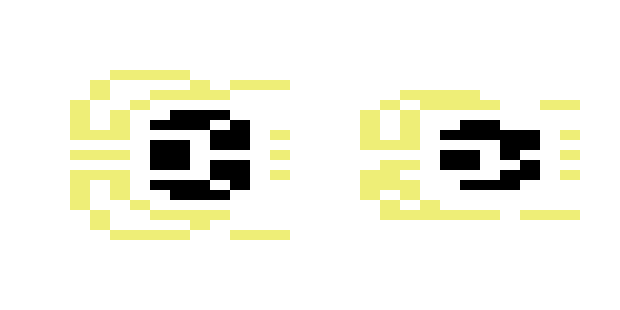
\includegraphics[height=0.6cm]{src/manta_spin/manta_spin_last_two_3.png}}
- rotates the ship to the opposite roll position.

\vspace{-0.5cm}
\begin{figure}[H]
    \centering
    \begin{adjustbox}{width=6cm,center}
      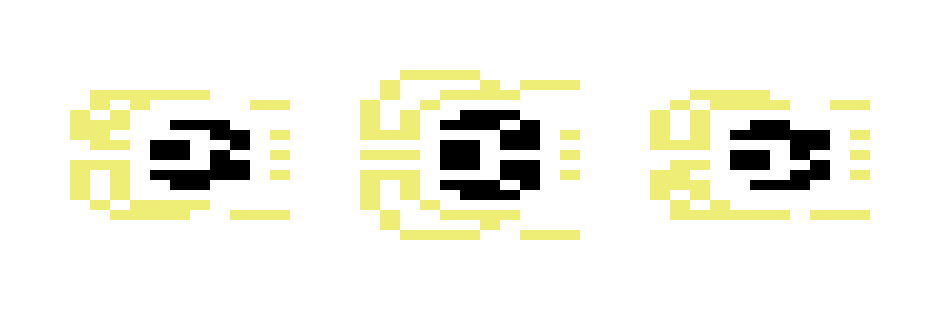
\includegraphics[width=15cm]{src/manta_spin/manta_spin_3.png}%
    \end{adjustbox}
\end{figure}
\vspace{-0.6cm}

So the Manta starts tilted away from us, rotates to a flat position, and then begins its roll towards
us. Notice the subtly different assymetry in the cockpit of the Manta when it is rolled away from us
compared to when it is rolled towards us. It is easiest to compare this difference in detail on the
following page where we blow up each of the tilted sprites to see how they are constructed from their
source data.

\begin{figure}[H]
    \centering
    \begin{adjustbox}{width=14cm,center}
      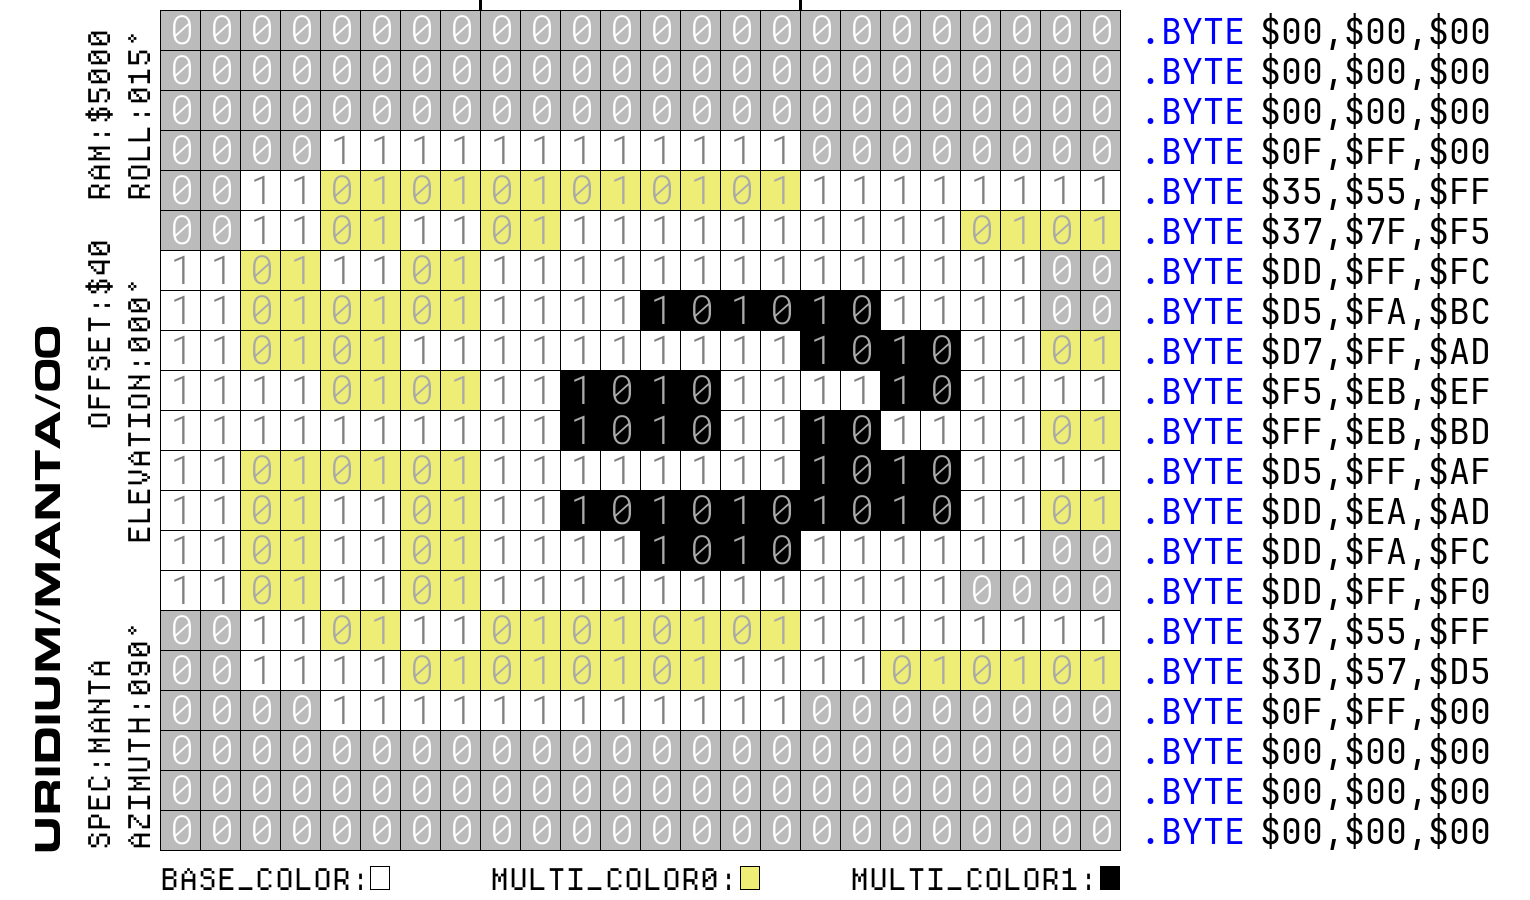
\includegraphics[width=15cm]{src/manta_diagrams_list/MANTA_0.png}%
    \end{adjustbox}
\end{figure}
\begin{figure}[H]
    \centering
    \begin{adjustbox}{width=14cm,center}
      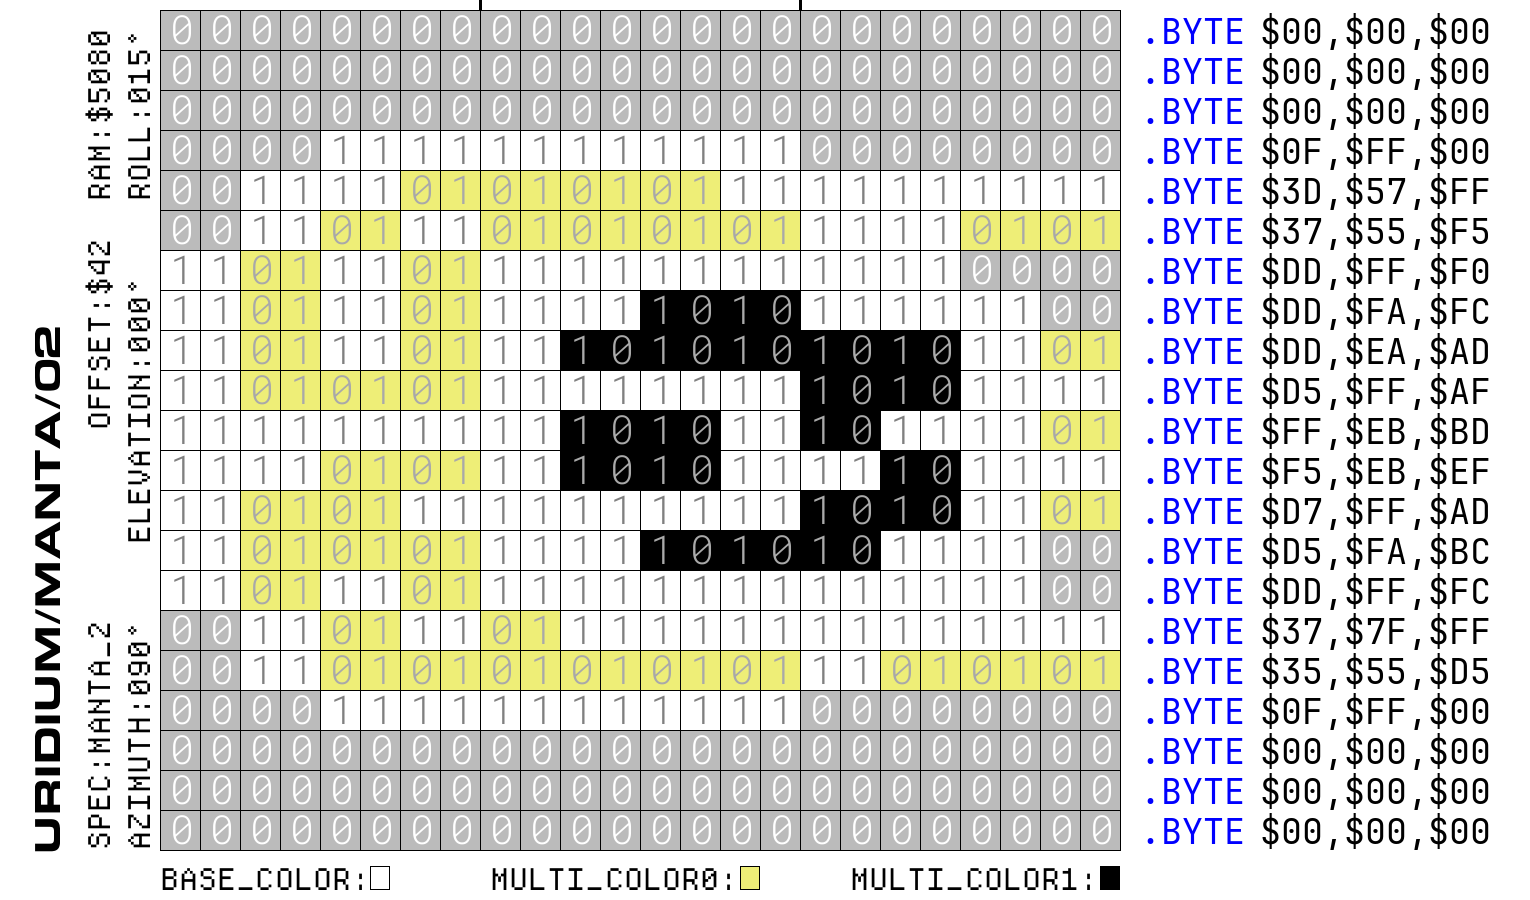
\includegraphics[width=15cm]{src/manta_diagrams_list/MANTA_2.png}%
    \end{adjustbox}
\end{figure}

Closer inspection reveals a simple trick that behind this detailing: the yellow and black regions have
simply had their order reversed and are mirror images of each other. For example if we take a look at
the region representing the cockpit:

\begin{minipage}[c]{0.48\linewidth}
\vspace{-0.5cm}
\begin{figure}[H]
    \centering
    \begin{adjustbox}{width=5cm,center}
      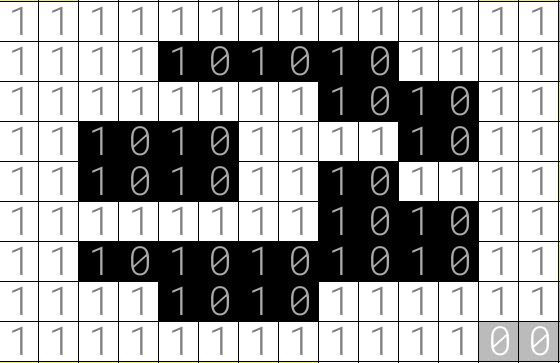
\includegraphics{src/manta_diagrams_list/MANTA_0_DETAIL.png}%
    \end{adjustbox}
\end{figure}
\end{minipage}
\begin{minipage}[c]{0.06\linewidth}
\begin{figure}[H]
    \centering
    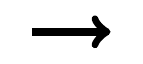
\begin{tikzpicture}[baseline={(current bounding box.south)}]
      \draw[->,line width=3pt] (0,0) to (1,0);
    \end{tikzpicture}
\end{figure}
\end{minipage}
\begin{minipage}[c]{0.48\linewidth}
\vspace{-0.5cm}
\begin{figure}[H]
    \centering
    \begin{adjustbox}{width=5cm,center}
      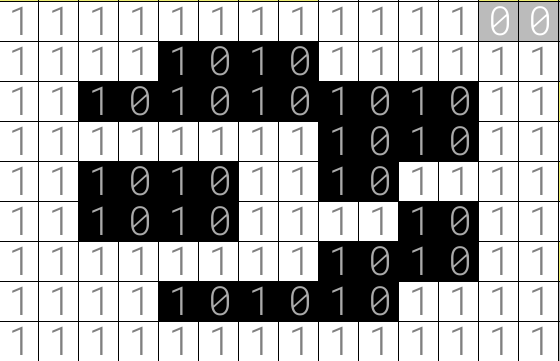
\includegraphics{src/manta_diagrams_list/MANTA_2_DETAIL.png}%
    \end{adjustbox}
\end{figure}
\end{minipage}

In its simplest terms the vertical order of the black lines detailing the cockpit have been reversed
and this alone is enough to suggest the difference in attitude along the Y co-ordinate.

Examining this detail may also give you a sense of how the sprites themselves are defined. In the diagram
above, for example, it may now be obvious that the black colour is defined by a bit pair of \icode{10} and
that the white colour is defined by a bit pair of \icode{11}. In the diagrams opposite, we can further see
that yellow is defined by the bit paid \icode{01} and the transparent background of the sprite by \icode{00}.

In the diagrams opposite and elsewhere we have given the three bytes that together make up the 12 bit pairs constituting
each of the 21 lines in the sprite, a total of 63 bytes in total. This is the source data used by \textit{Uridium's} 6502
assembler code to build each sprite using the straightforward process of mapping each bit pair to a corresponding
pair of coloured pixels. An important feature of this sprite data is that it is stored contiguously for all sprites in the computer's
RAM, or memory area, starting at address \icode{\$5000}. This is important because the order in which the sprite
data is stored corresponds exactly to the order of each frame in the manta spin animation. 

We can get a better sense of this by observing the RAM address of each sprite in the section of animation sequence
between the ship faced towards and faced away. The first sprite in the sequence is at address \icode{\$5040}, the second
at \icode{\$5080}, and so on. At each step, to get the next frame in the animation all that has to be done is to 
increment the position in RAM we are adressing by \icode{\$40}.

\begin{figure}[H]
    \centering
    \begin{adjustbox}{width=13.5cm,center}
      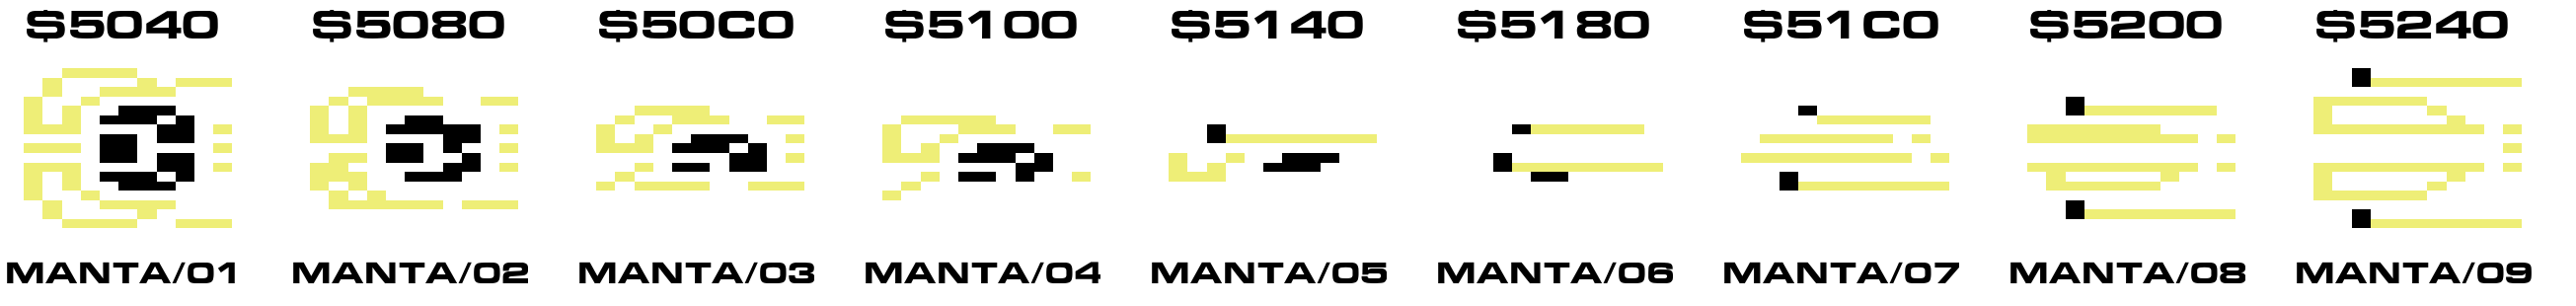
\includegraphics[width=15cm]{src/manta_spin/manta_spin_first_half.png}%
    \end{adjustbox}
\end{figure}
\vspace{-0.6cm}

\begin{figure}[H]
    \centering
    \begin{adjustbox}{width=14cm,center}
      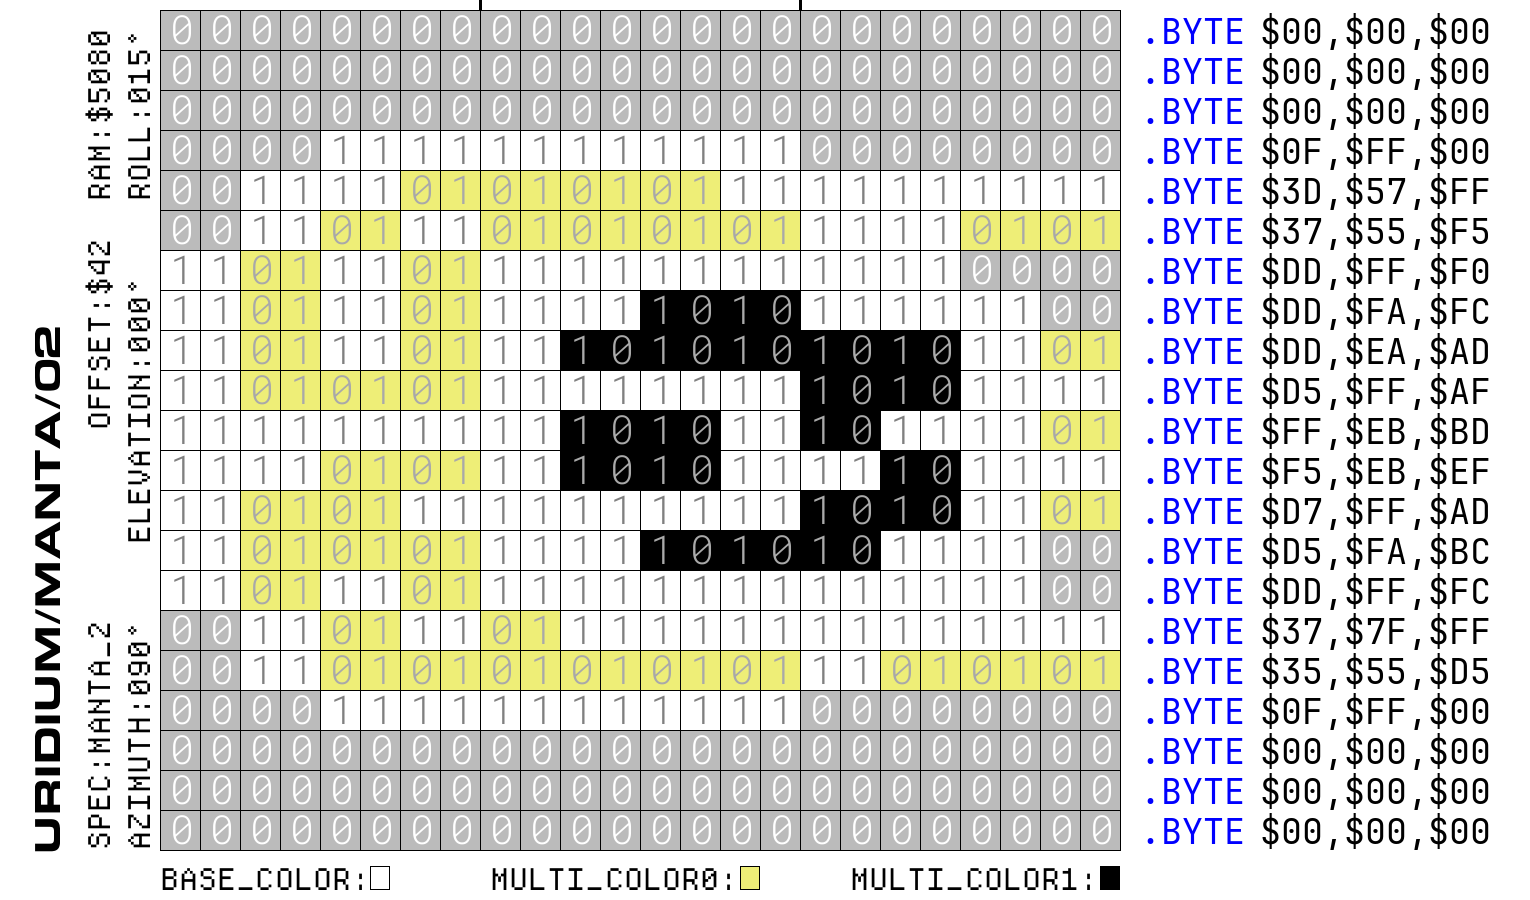
\includegraphics[width=7cm]{src/manta_diagrams_list/MANTA_2.png}%
      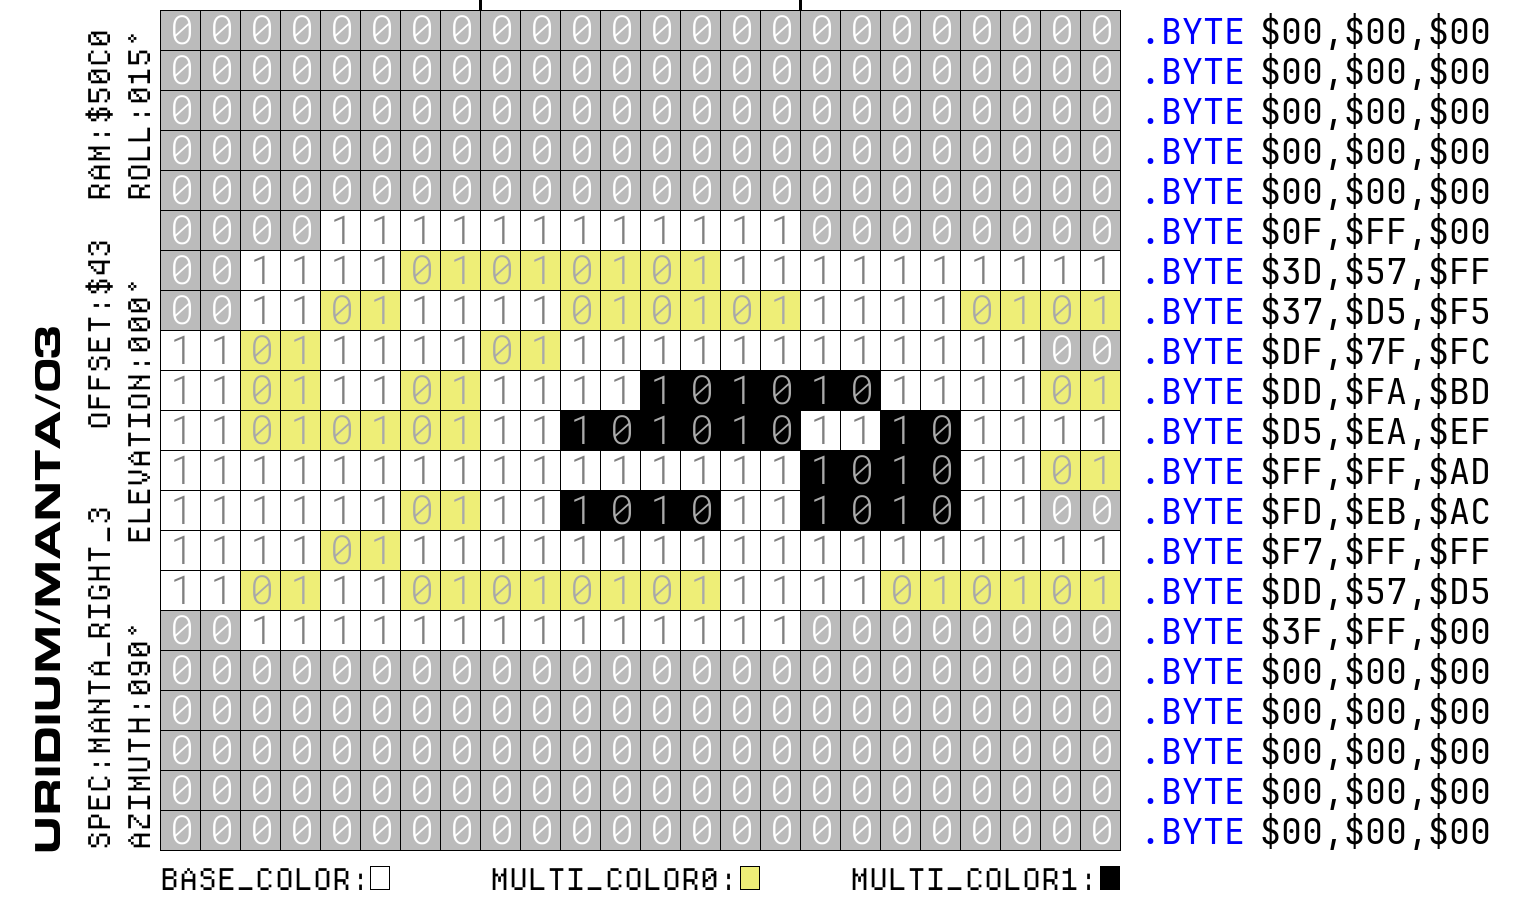
\includegraphics[width=7cm]{src/manta_diagrams_list/MANTA_3.png}%
    \end{adjustbox}
\end{figure}
\vspace{-0.5cm}
\begin{figure}[H]
    \centering
    \begin{adjustbox}{width=14cm,center}
      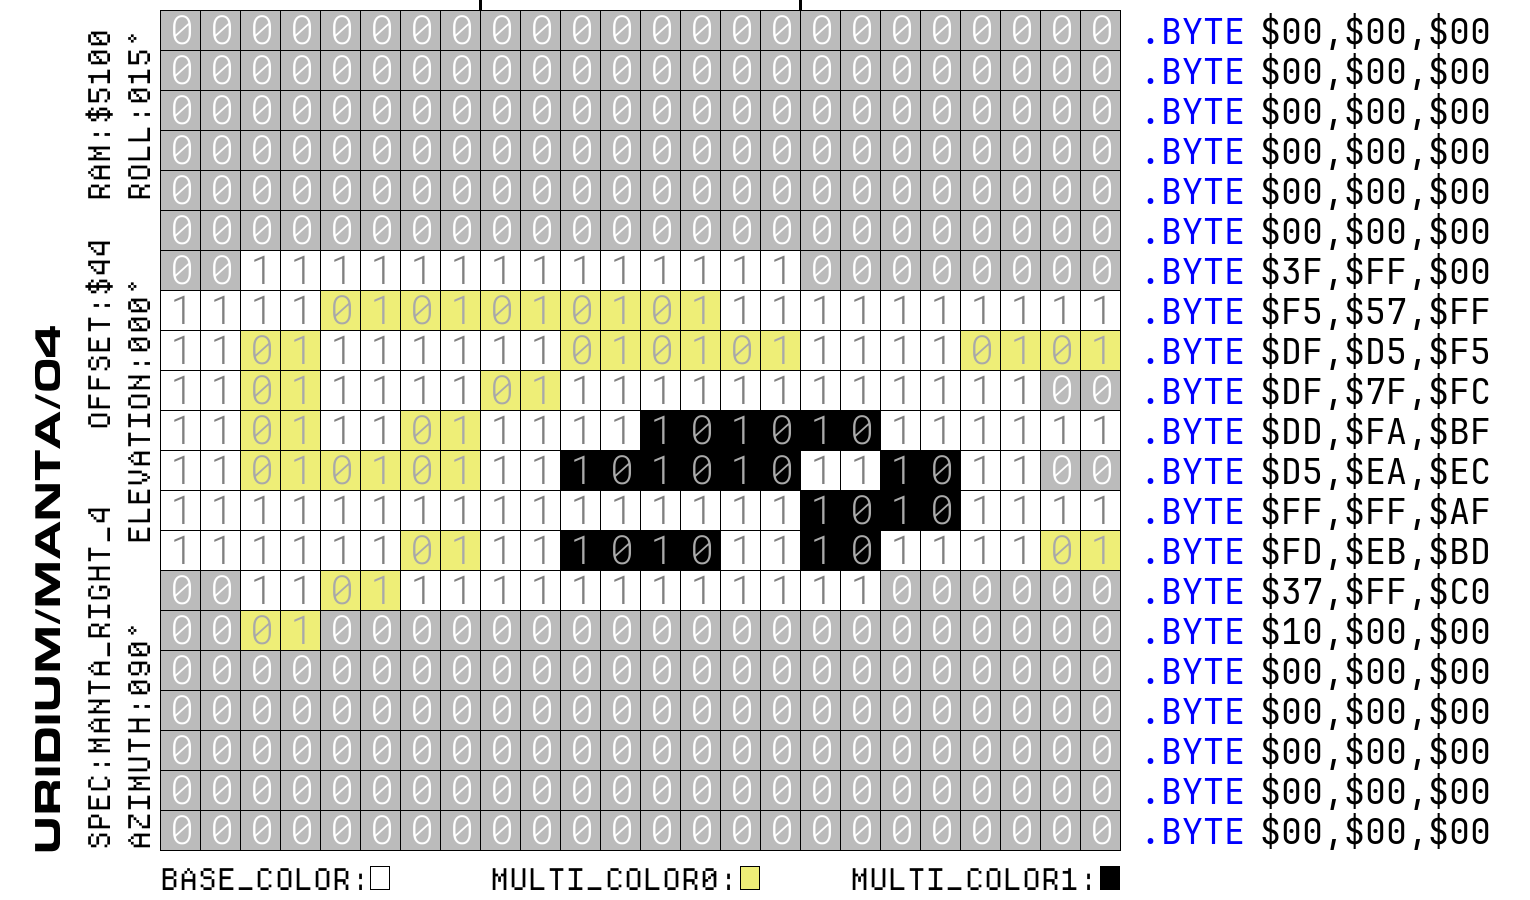
\includegraphics[width=7cm]{src/manta_diagrams_list/MANTA_4.png}%
      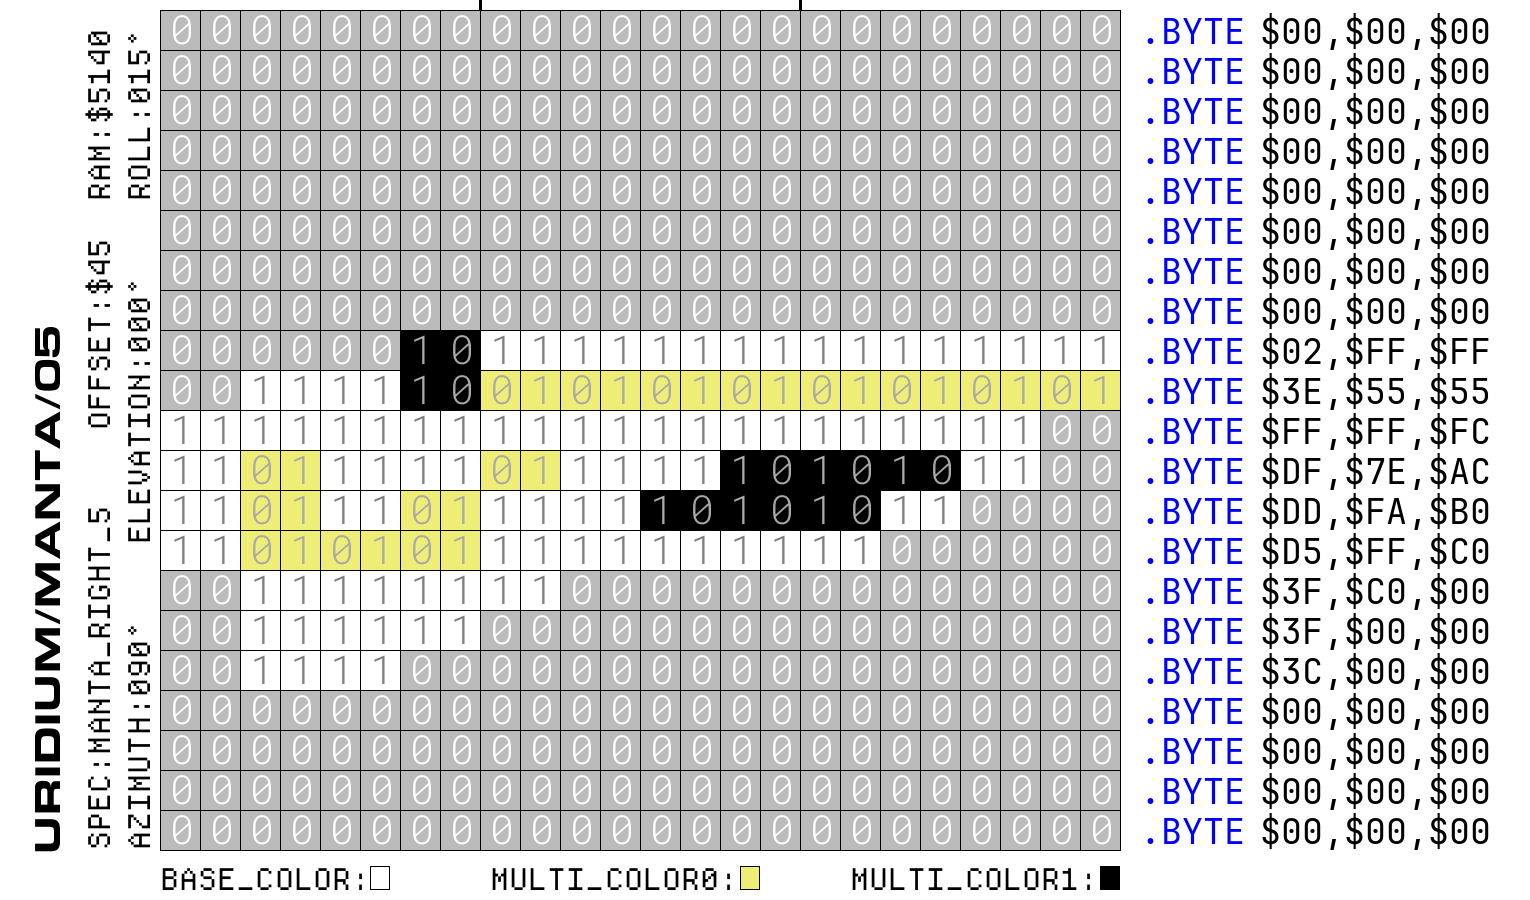
\includegraphics[width=7cm]{src/manta_diagrams_list/MANTA_5.png}%
    \end{adjustbox}
\end{figure}
\vspace{-0.5cm}
\begin{figure}[H]
    \centering
    \begin{adjustbox}{width=14cm,center}
      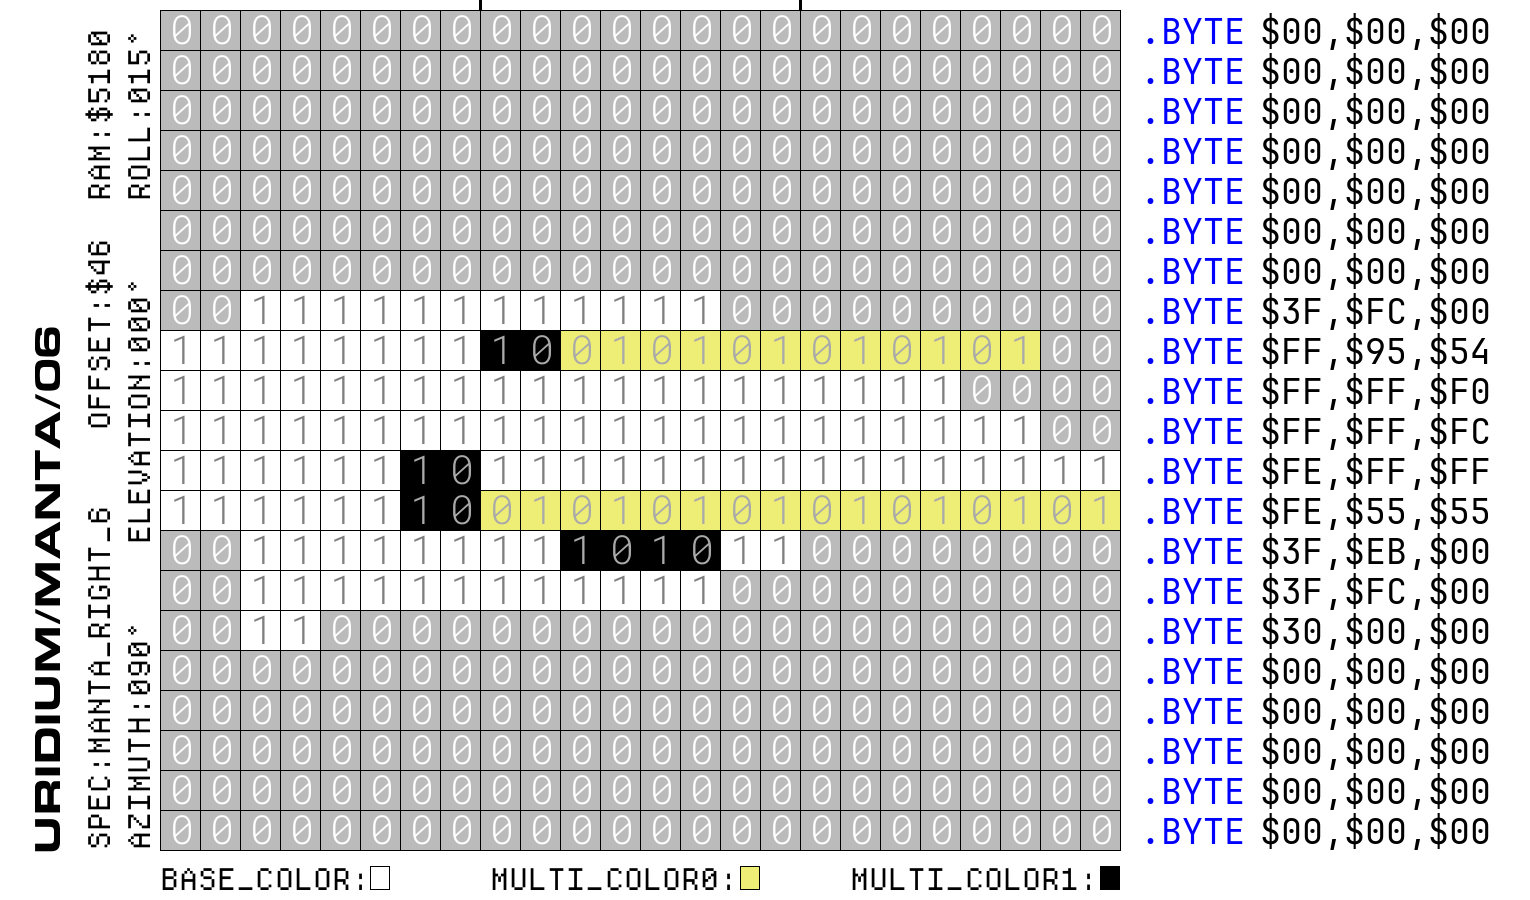
\includegraphics[width=7cm]{src/manta_diagrams_list/MANTA_6.png}%
      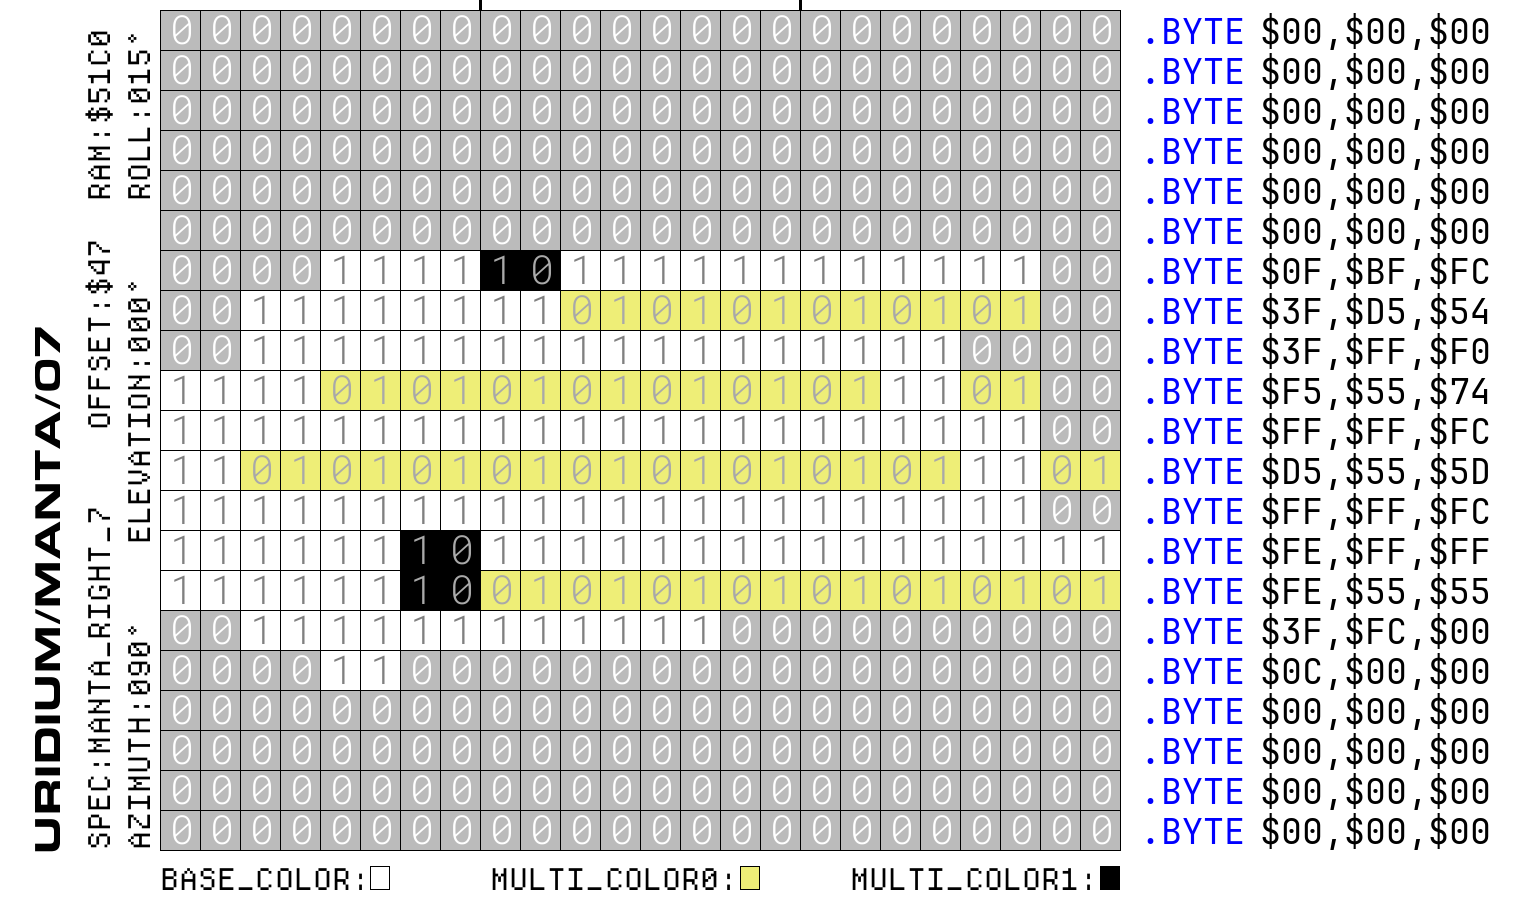
\includegraphics[width=7cm]{src/manta_diagrams_list/MANTA_7.png}%
    \end{adjustbox}
\end{figure}
\vspace{-0.5cm}
\begin{figure}[H]
    \centering
    \begin{adjustbox}{width=14cm,center}
      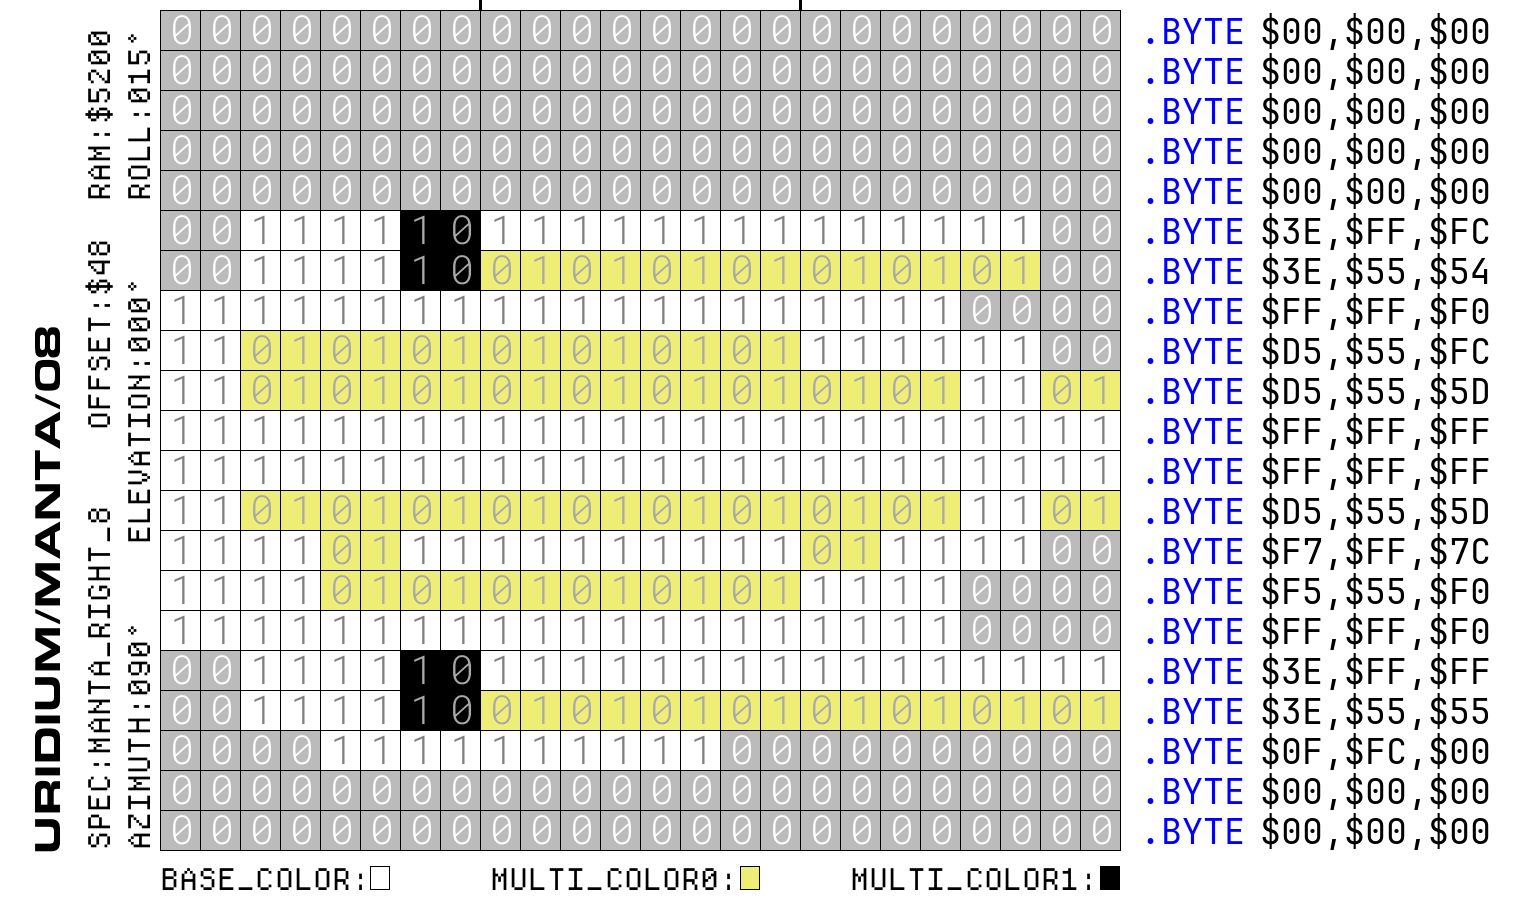
\includegraphics[width=7cm]{src/manta_diagrams_list/MANTA_8.png}%
      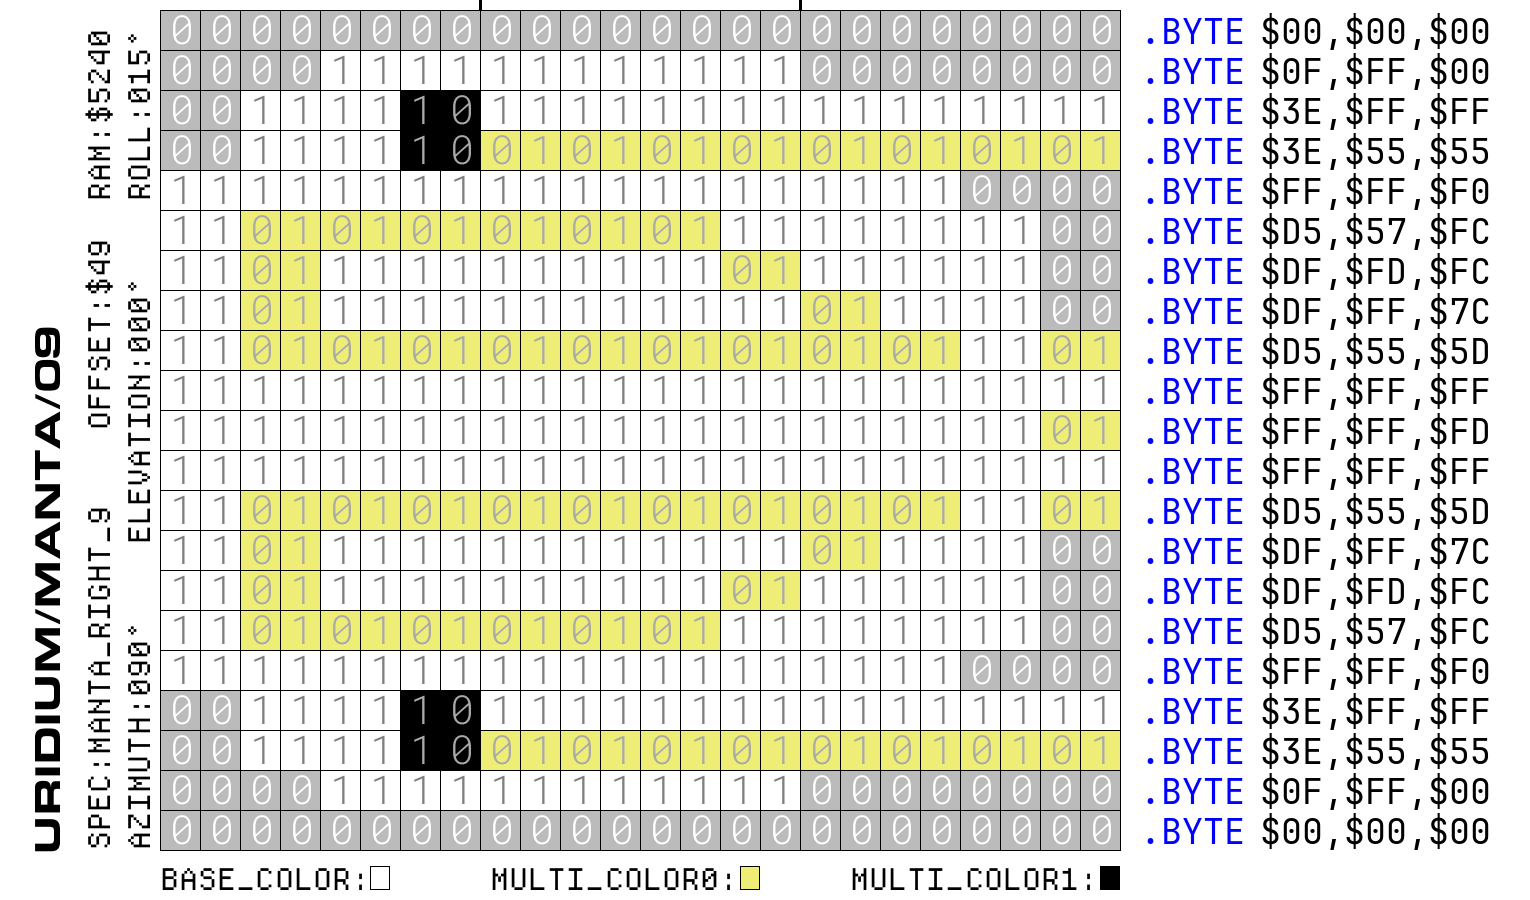
\includegraphics[width=7cm]{src/manta_diagrams_list/MANTA_9.png}%
    \end{adjustbox}
\end{figure}

This approach does not hold for the second half of the animation sequence, or at least
not all of it. As we can see below, the final two frames of the sequence reset back
to address \icode{\$5000} to stitch in the start of the animation and complete the
loop.
\begin{figure}[H]
    \centering
    \begin{adjustbox}{width=13.5cm,center}
      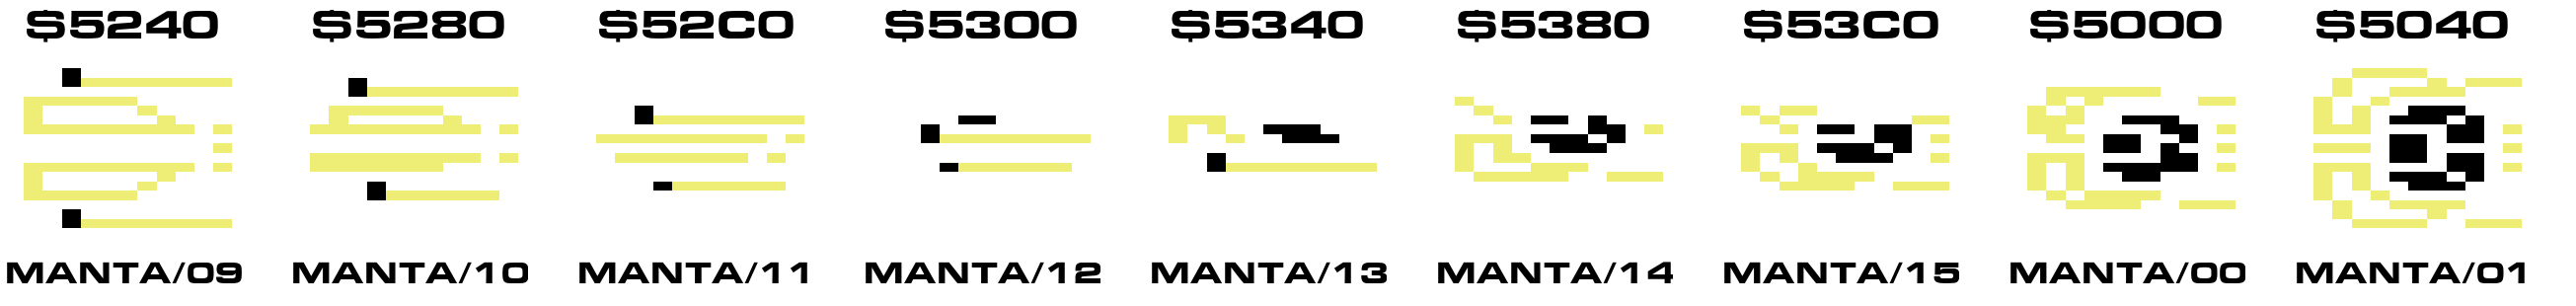
\includegraphics[width=15cm]{src/manta_spin/manta_spin_second_half.png}%
    \end{adjustbox}
\end{figure}
\vspace{-0.6cm}



\begin{lstlisting}
SpinningShipAnimationLoop
        JSR CheckInputMaybeUpdateDecal
        LDA firePressed
        BEQ SpinningShipAnimationOver
        LDA someKindOfFrameRate
        BEQ SpinningShipAnimationOver
        JSR MaybeShowPauseScreen
        JSR StoreSpriteContentColorAndPosition
        INC currentSpriteValue
        LDA currentSpriteValue
        CMP #MANTA_16
        BCC Repeat
        LDA #MANTA_00
        STA currentSpriteValue
Repeat  JSR UpdateSpriteContentAndPosition
        JMP SpinningShipAnimationLoop
\end{lstlisting}

\begin{figure}[H]
    \centering
    \begin{adjustbox}{width=14cm,center}
      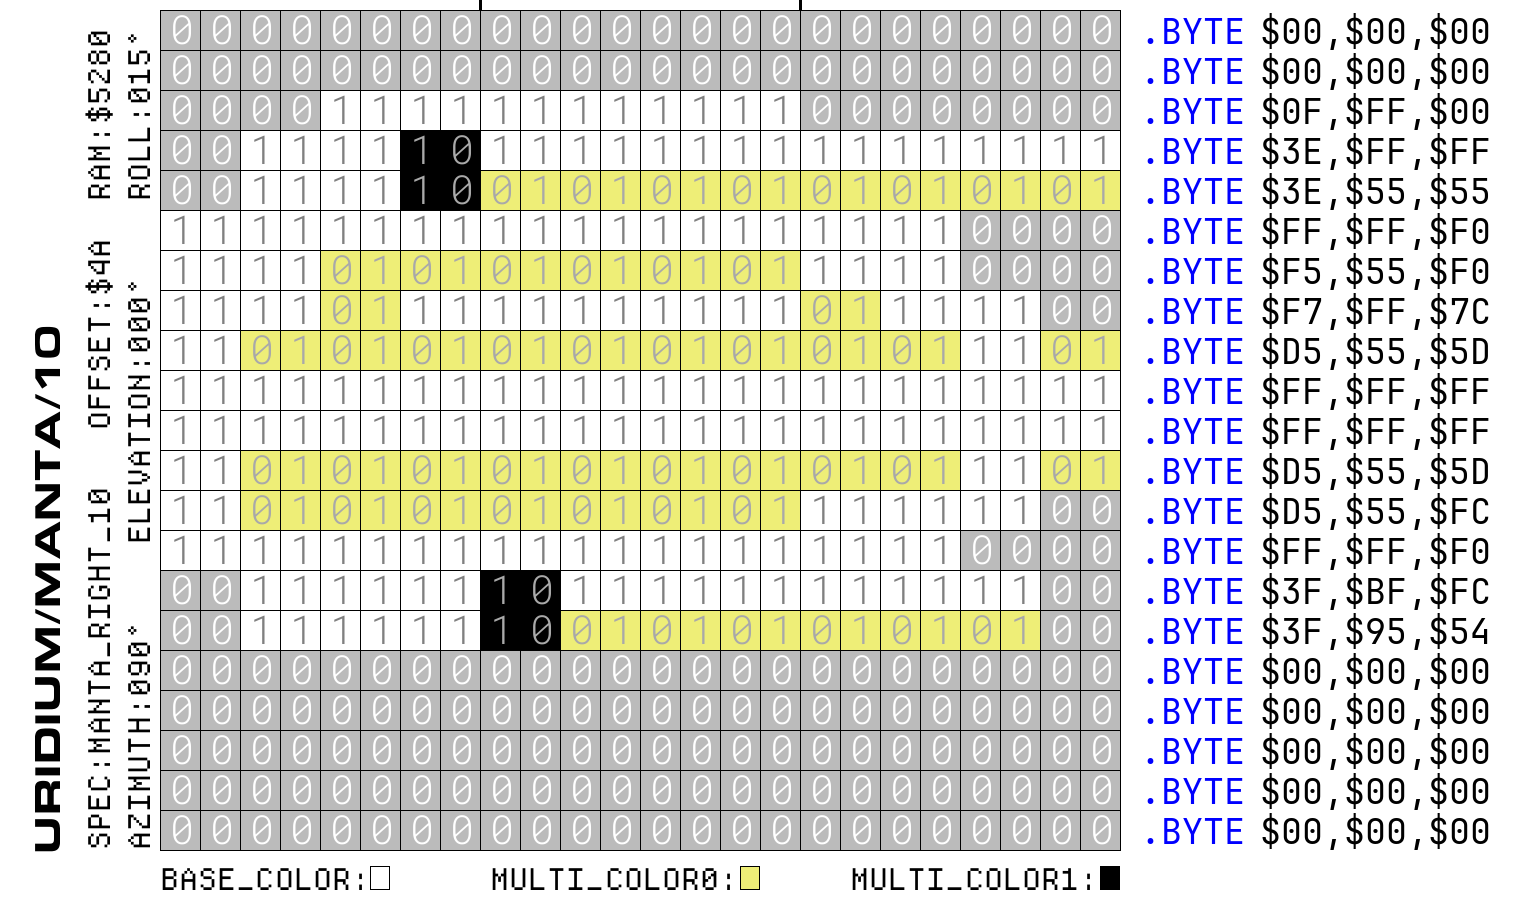
\includegraphics[width=7cm]{src/manta_diagrams_list/MANTA_10.png}%
      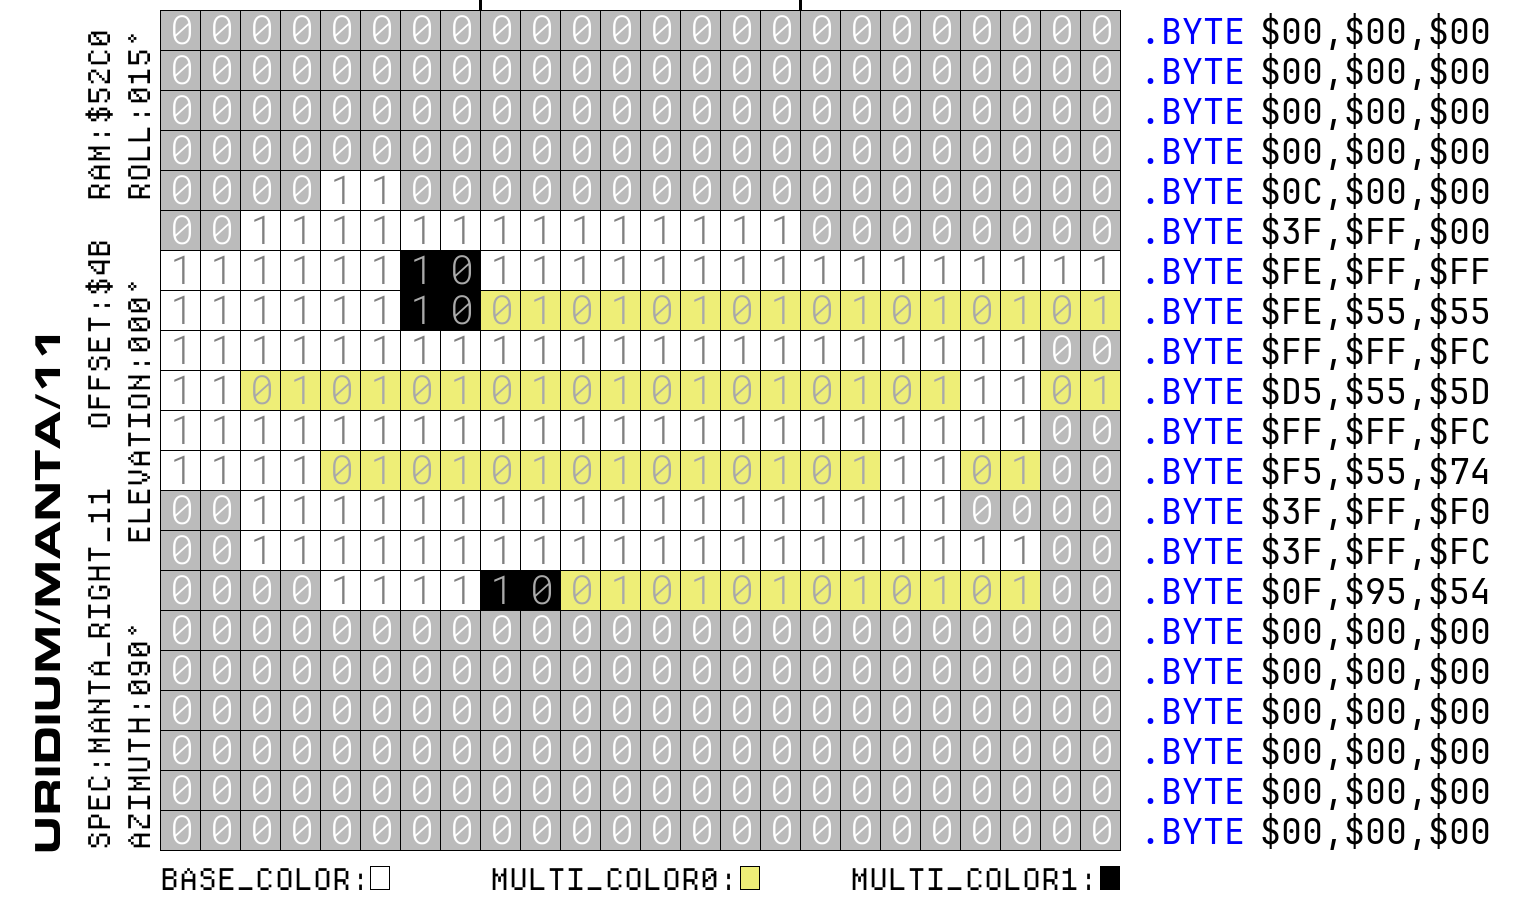
\includegraphics[width=7cm]{src/manta_diagrams_list/MANTA_11.png}%
    \end{adjustbox}
\end{figure}
\vspace{-0.5cm}
\begin{figure}[H]
    \centering
    \begin{adjustbox}{width=14cm,center}
      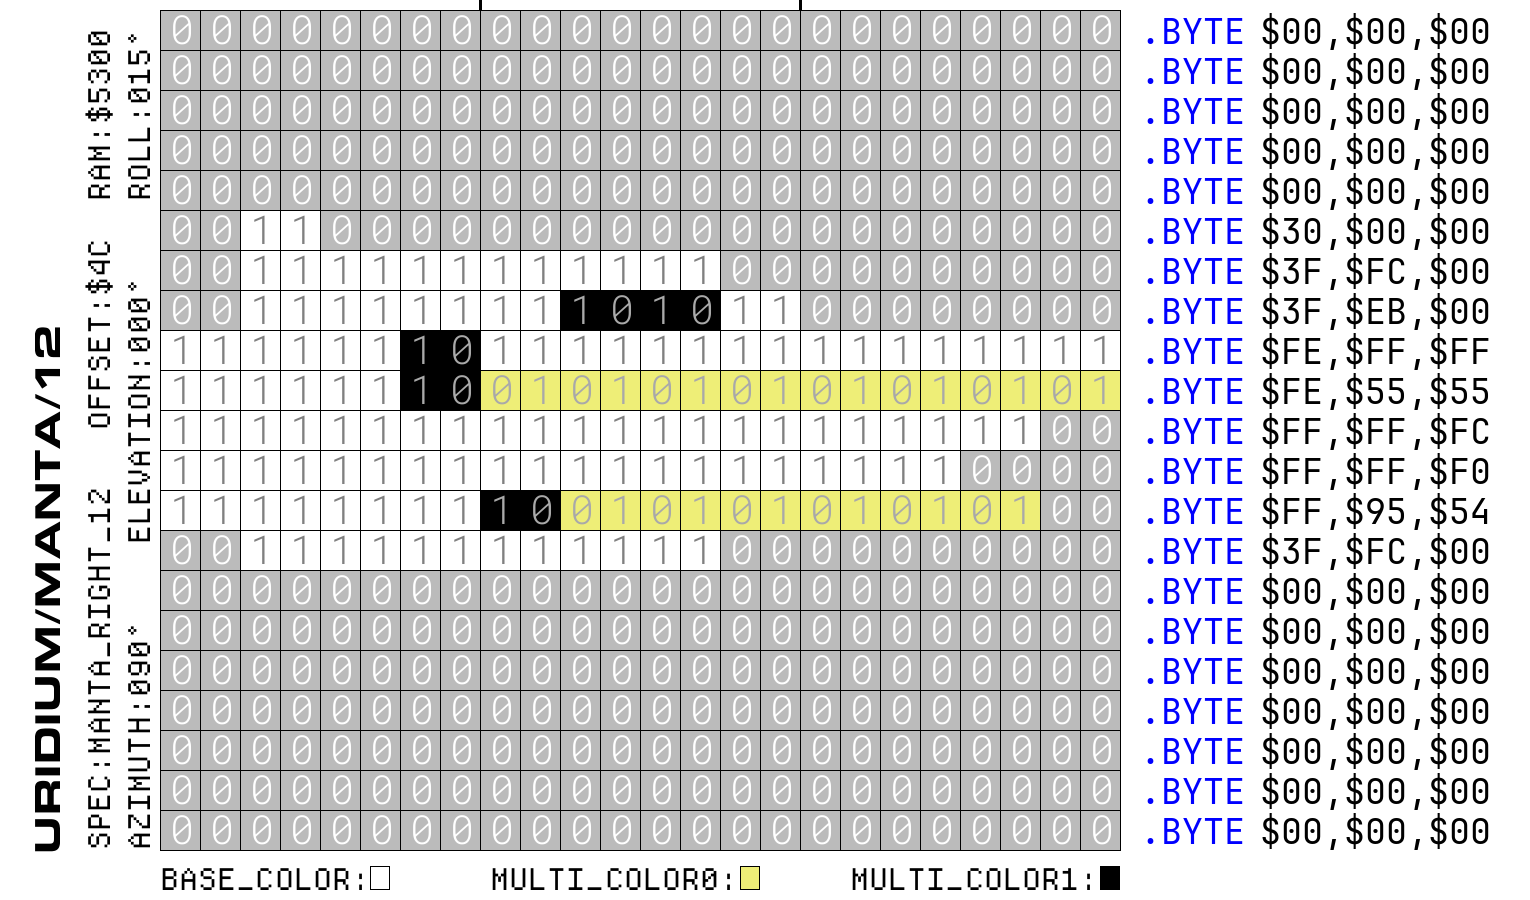
\includegraphics[width=7cm]{src/manta_diagrams_list/MANTA_12.png}%
      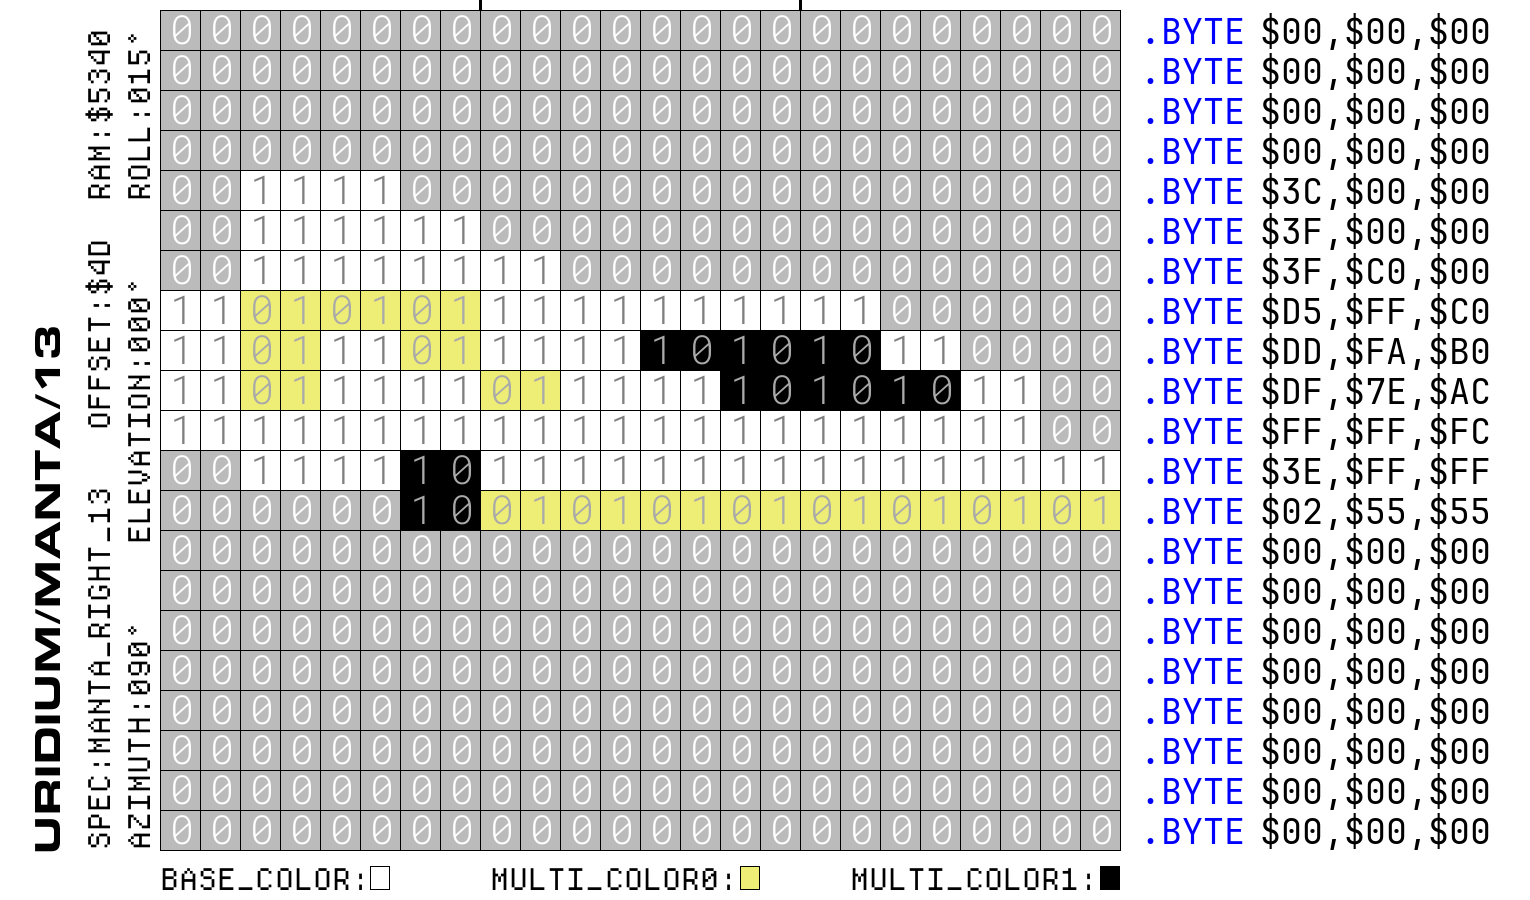
\includegraphics[width=7cm]{src/manta_diagrams_list/MANTA_13.png}%
    \end{adjustbox}
\end{figure}
\vspace{-0.5cm}
\begin{figure}[H]
    \centering
    \begin{adjustbox}{width=14cm,center}
      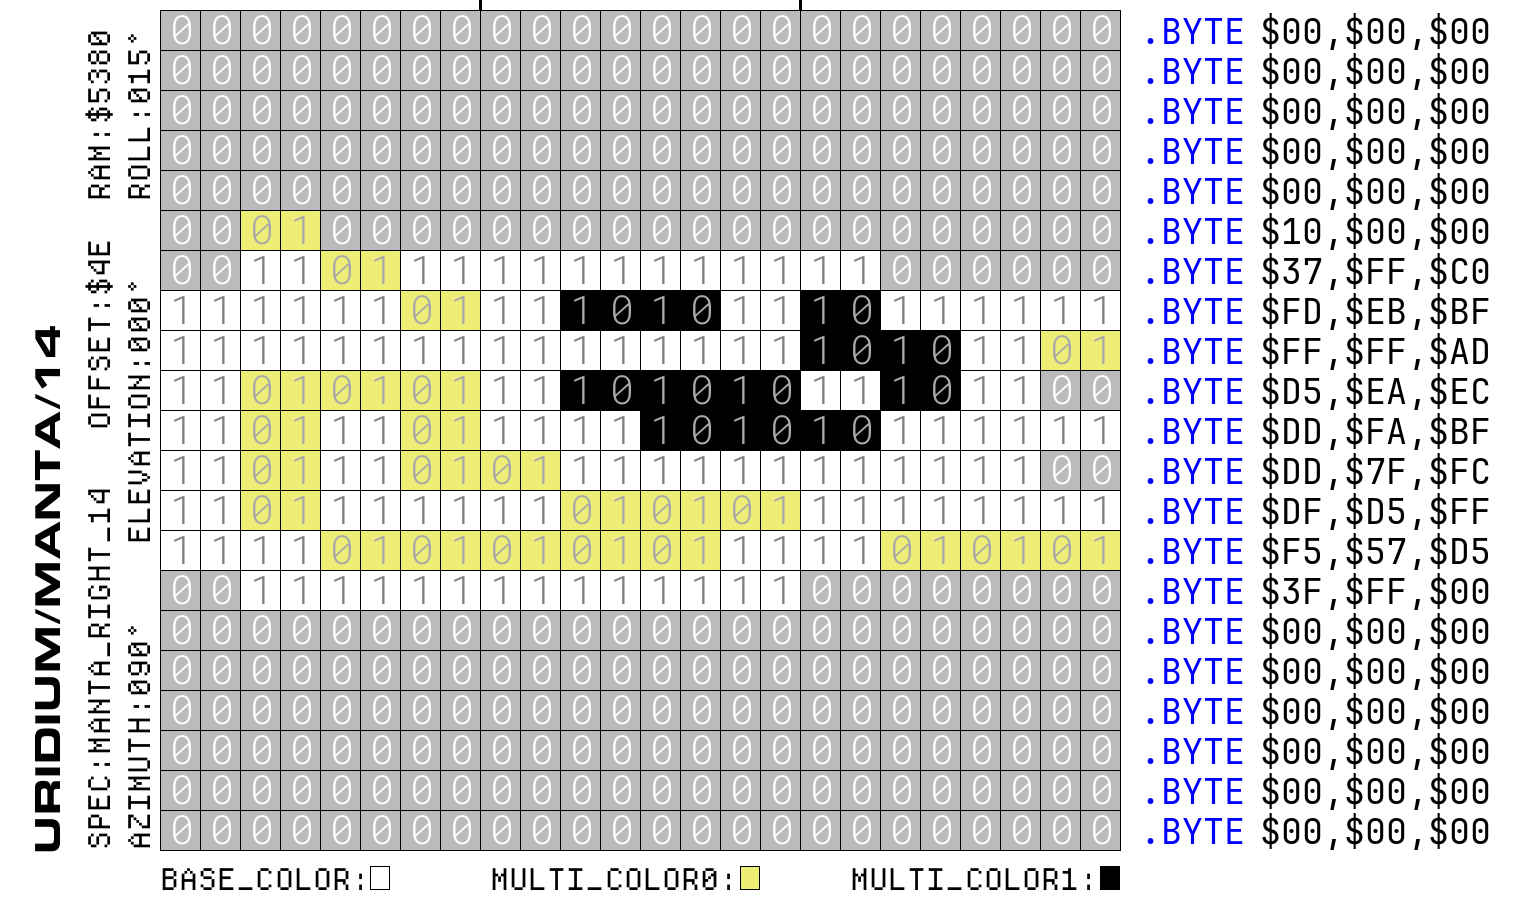
\includegraphics[width=7cm]{src/manta_diagrams_list/MANTA_14.png}%
      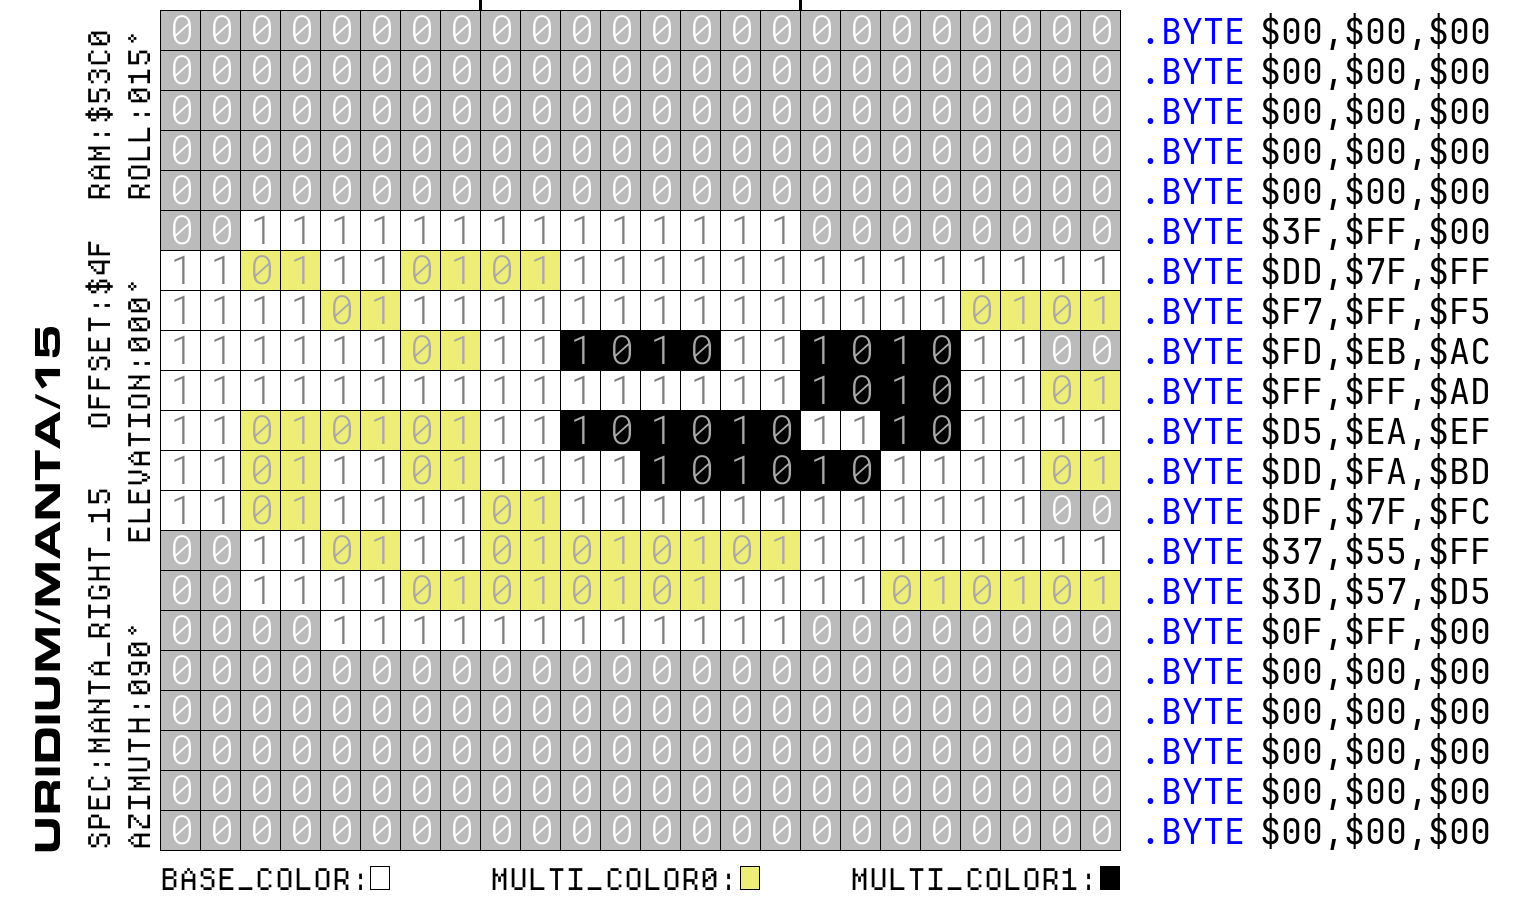
\includegraphics[width=7cm]{src/manta_diagrams_list/MANTA_15.png}%
    \end{adjustbox}
\end{figure}
\vspace{-0.5cm}
\begin{figure}[H]
    \centering
    \begin{adjustbox}{width=14cm,center}
      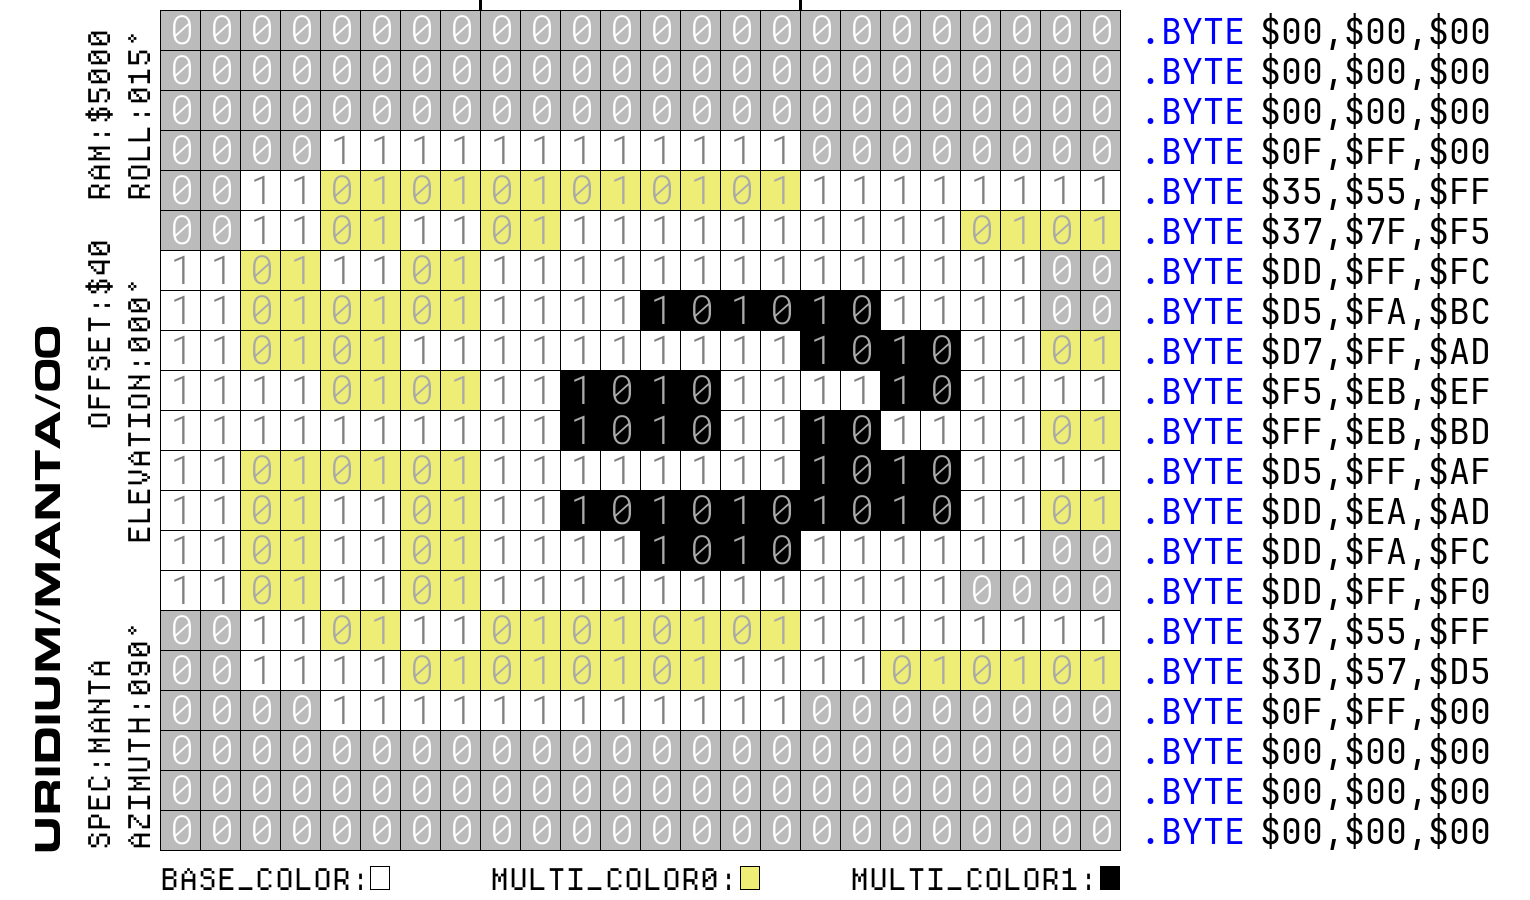
\includegraphics[width=7cm]{src/manta_diagrams_list/MANTA_0.png}%
      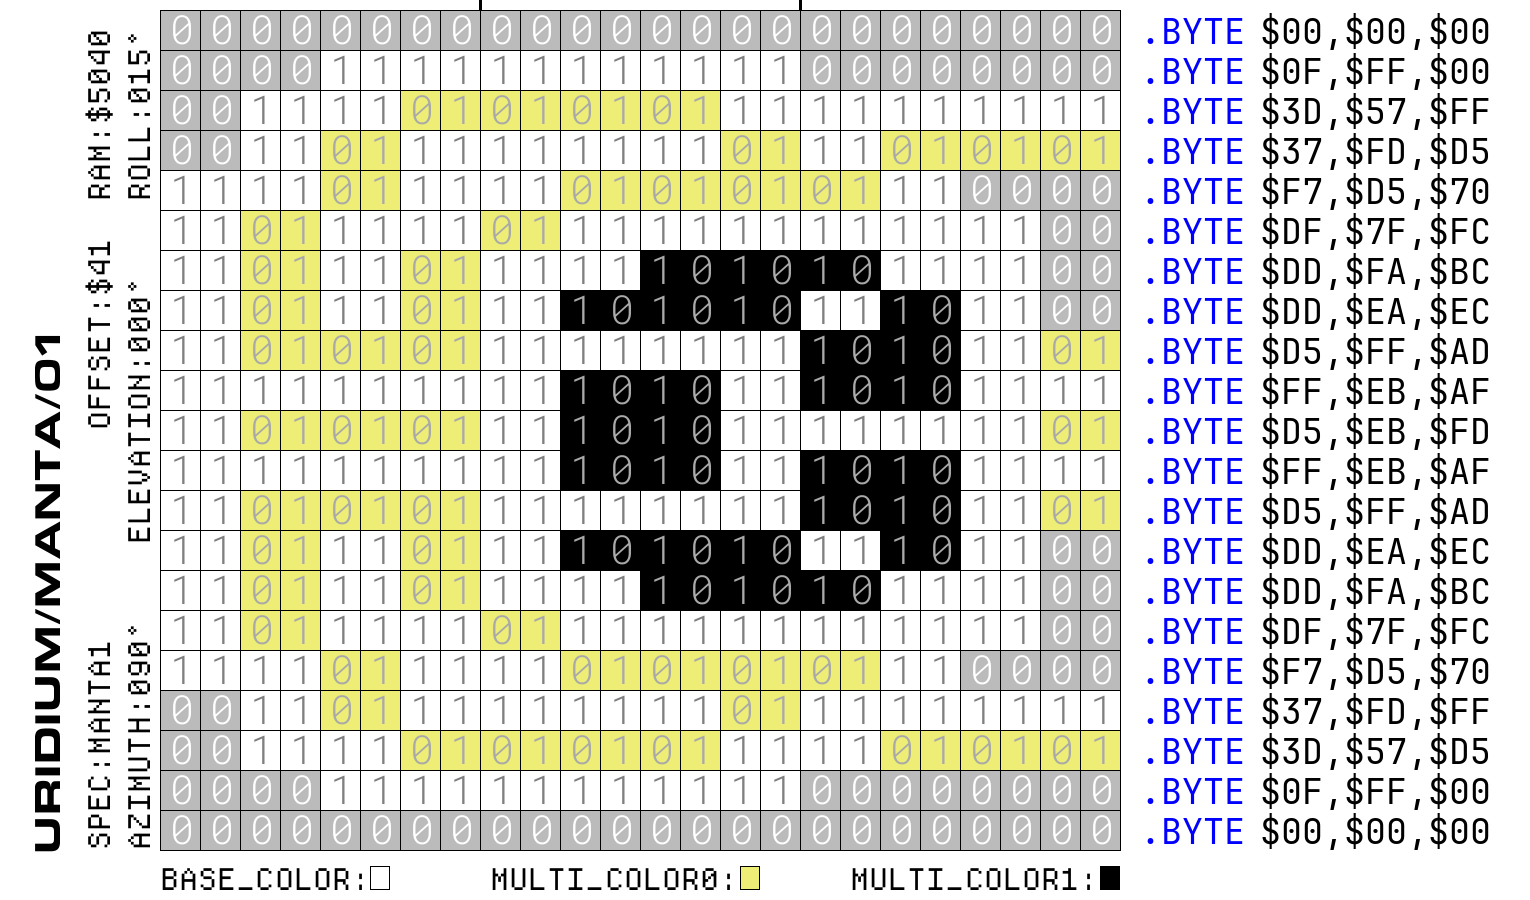
\includegraphics[width=7cm]{src/manta_diagrams_list/MANTA_1.png}%
    \end{adjustbox}
\end{figure}
